\documentclass[crop,border=7pt]{standalone}
\usepackage{tikz}
\usepackage{ifthen}
\usetikzlibrary{shapes.geometric}
\begin{document}
  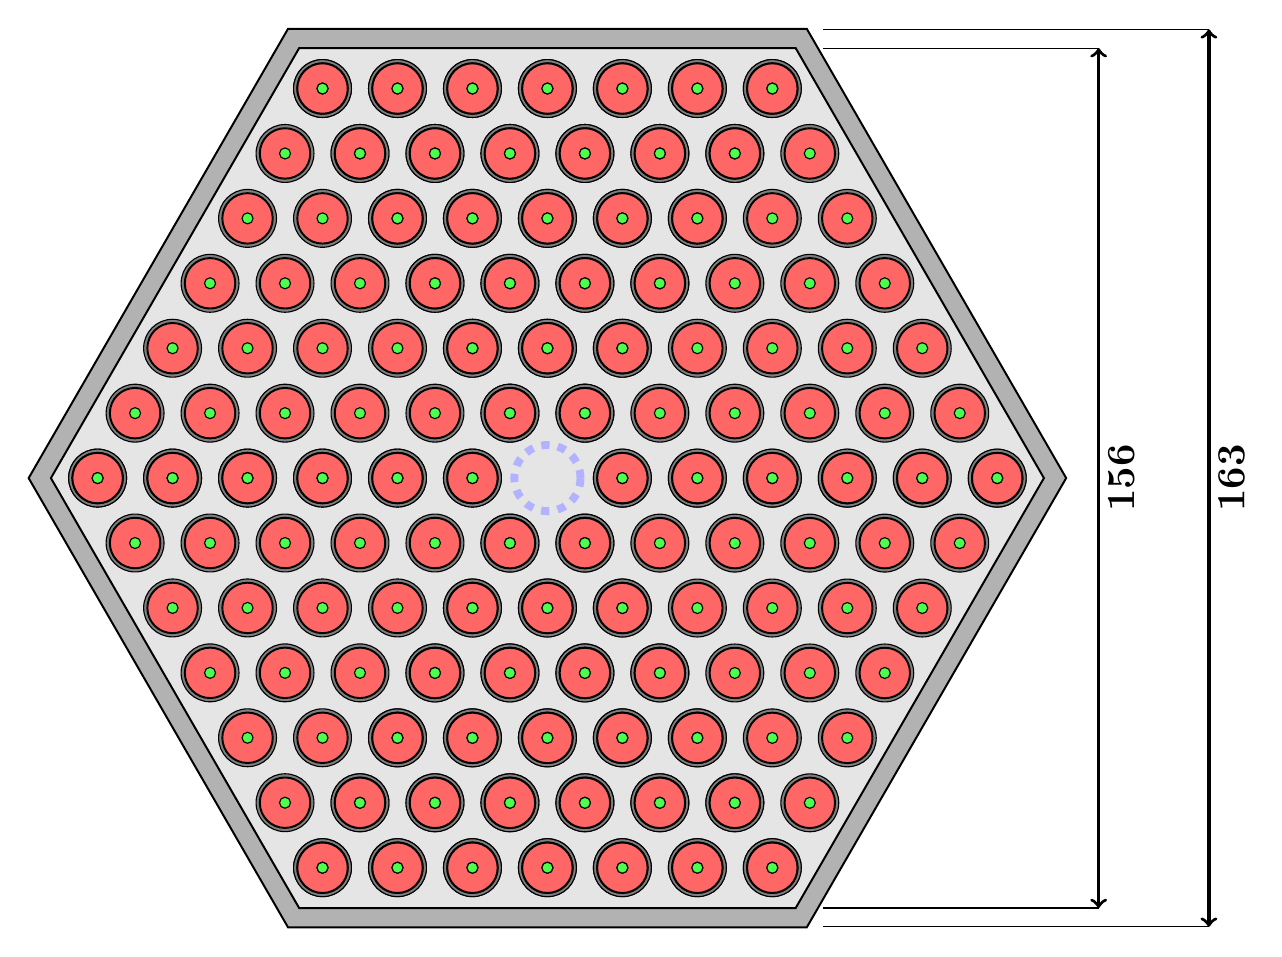
\begin{tikzpicture}[scale=0.07]
%%%%%%%%%

\draw[black, thin] (50,81.4064) - - (120,81.4064);
\draw[black, thin] (50,-81.4064) - - (120,-81.4064);
\draw[black, very thick, <->] (120,-81.4064) -- (120,81.4064);
\draw[black] (120,0) node[anchor=north, rotate=90] {\Large \textbf{163}};

%%%%%%%%%%%%%%%%%%%%%%
\draw[black, thin] (50,78.0003) - - (100,78.0003);
\draw[black, thin] (50,-78.0003) - - (100,-78.0003);
\draw[black, very thick, <->] (100,-78.0003) -- (100,78.0003);
\draw[black] (100,0) node[anchor=north, rotate=90] {\Large \textbf{156}};
%%%hexagon 1
\newdimen\R
\R=94.108cm
  \coordinate (center) at (0,0);
 \filldraw[gray!60, draw=black,line width=0.25mm] (0:\R)
     \foreach \x in {60,120,...,360} {  -- (\x:\R) }
              -- cycle (300:\R)
              -- cycle (240:\R) 
              -- cycle (180:\R) 
              -- cycle (120:\R) 
              -- cycle (60:\R) 
              -- cycle (0:\R) ;
%%%%%%%%%
%%%hexagon 2
\newdimen\R
\R=90.07cm
  \coordinate (center) at (0,0);
 \filldraw[gray!20, draw=black,line width=0.25mm] (0:\R)
     \foreach \x in {60,120,...,360} {  -- (\x:\R) }
              -- cycle (300:\R)
              -- cycle (240:\R) 
              -- cycle (180:\R) 
              -- cycle (120:\R) 
              -- cycle (60:\R) 
              -- cycle (0:\R) ;
%%%%%%%%%firstloop circle
\foreach[evaluate={\y=-70.668+11.778*\t}] \t in {0,...,6}
\foreach[evaluate={\xi=-40.8-6.8*\t}] \l in {1,...,1}
\foreach[evaluate={\x=\xi+13.6*\r}] \r in {0,...,6}
			\filldraw[gray, draw=black] (\x,\y) circle (5.25cm);
%			\filldraw[green!70, draw=black] (\x,\y) circle (4.65cm);
%			\filldraw[red!60, draw=black] (\x,\y) circle (4.5cm);
%			\filldraw[green!70, draw=black] (\x,\y) circle (1.0cm);
\foreach[evaluate={\y=11.778*\t}] \t in {0,...,6}
\foreach[evaluate={\xi=-81.6+6.8*\t}] \l in {1,...,1}
\foreach[evaluate={\x=\xi+13.6*\r}] \r in {0,...,6}
			\filldraw[gray, draw=black] (\x,\y) circle (5.25cm);
%			\filldraw[green!70, draw=black] (\x,\y) circle (4.65cm);
%			\filldraw[red!60, draw=black] (\x,\y) circle (4.5cm);
%			\filldraw[green!70, draw=black] (\x,\y) circle (1.0cm);
\foreach[evaluate={\y=-70.688+11.778*\t}] \t in {0,...,6}
\foreach[evaluate={\xi=-40.8+6.8*\t}] \l in {1,...,1}
\foreach[evaluate={\x=\xi+13.6*\r}] \r in {0,...,6}
			\filldraw[gray, draw=black] (\x,\y) circle (5.25cm);
%			\filldraw[green!70, draw=black] (\x,\y) circle (4.65cm);
%			\filldraw[red!60, draw=black] (\x,\y) circle (4.5cm);
%			\filldraw[green!70, draw=black] (\x,\y) circle (1.0cm);
\foreach[evaluate={\y=11.778*\t}] \t in {0,...,6}
\foreach[evaluate={\xi=81.6-6.8*\t}] \l in {1,...,1}
\foreach[evaluate={\x=\xi-13.6*\r}] \r in {0,...,6}
			\filldraw[gray, draw=black] (\x,\y) circle (5.25cm);
%			\filldraw[green!70, draw=black] (\x,\y) circle (4.65cm);
%			\filldraw[red!60, draw=black] (\x,\y) circle (4.5cm);
%			\filldraw[green!70, draw=black] (\x,\y) circle (1.0cm);
              
              
              
              %%%%%%%%%second loop circle
\foreach[evaluate={\y=-70.668+11.778*\t}] \t in {0,...,6}
\foreach[evaluate={\xi=-40.8-6.8*\t}] \l in {1,...,1}
\foreach[evaluate={\x=\xi+13.6*\r}] \r in {0,...,6}
			\filldraw[green!70, draw=black] (\x,\y) circle (4.65cm);

\foreach[evaluate={\y=11.778*\t}] \t in {0,...,6}
\foreach[evaluate={\xi=-81.6+6.8*\t}] \l in {1,...,1}
\foreach[evaluate={\x=\xi+13.6*\r}] \r in {0,...,6}
			\filldraw[green!70, draw=black] (\x,\y) circle (4.65cm);
			
\foreach[evaluate={\y=-70.688+11.778*\t}] \t in {0,...,6}
\foreach[evaluate={\xi=-40.8+6.8*\t}] \l in {1,...,1}
\foreach[evaluate={\x=\xi+13.6*\r}] \r in {0,...,6}
			\filldraw[green!70, draw=black] (\x,\y) circle (4.65cm);
			
\foreach[evaluate={\y=11.778*\t}] \t in {0,...,6}
\foreach[evaluate={\xi=81.6-6.8*\t}] \l in {1,...,1}
\foreach[evaluate={\x=\xi-13.6*\r}] \r in {0,...,6}
			\filldraw[green!70, draw=black] (\x,\y) circle (4.65cm);
			
			
			
			%%%%%third loop circle
			%%%%%%%%%firstloop circle
\foreach[evaluate={\y=-70.668+11.778*\t}] \t in {0,...,6}
\foreach[evaluate={\xi=-40.8-6.8*\t}] \l in {1,...,1}
\foreach[evaluate={\x=\xi+13.6*\r}] \r in {0,...,6}
			\filldraw[red!60, draw=black] (\x,\y) circle (4.5cm);
			
\foreach[evaluate={\y=11.778*\t}] \t in {0,...,6}
\foreach[evaluate={\xi=-81.6+6.8*\t}] \l in {1,...,1}
\foreach[evaluate={\x=\xi+13.6*\r}] \r in {0,...,6}
			\filldraw[red!60, draw=black] (\x,\y) circle (4.5cm);
			
\foreach[evaluate={\y=-70.688+11.778*\t}] \t in {0,...,6}
\foreach[evaluate={\xi=-40.8+6.8*\t}] \l in {1,...,1}
\foreach[evaluate={\x=\xi+13.6*\r}] \r in {0,...,6}
			\filldraw[red!60, draw=black] (\x,\y) circle (4.5cm);
\foreach[evaluate={\y=11.778*\t}] \t in {0,...,6}
\foreach[evaluate={\xi=81.6-6.8*\t}] \l in {1,...,1}
\foreach[evaluate={\x=\xi-13.6*\r}] \r in {0,...,6}
			\filldraw[red!60, draw=black] (\x,\y) circle (4.5cm);
			
			
			
			%%%%%fourth loop circle
			%%%%%%%%%firstloop circle
\foreach[evaluate={\y=-70.668+11.778*\t}] \t in {0,...,6}
\foreach[evaluate={\xi=-40.8-6.8*\t}] \l in {1,...,1}
\foreach[evaluate={\x=\xi+13.6*\r}] \r in {0,...,6}
			\filldraw[green!70, draw=black] (\x,\y) circle (1.0cm);
			
\foreach[evaluate={\y=11.778*\t}] \t in {0,...,6}
\foreach[evaluate={\xi=-81.6+6.8*\t}] \l in {1,...,1}
\foreach[evaluate={\x=\xi+13.6*\r}] \r in {0,...,6}
			\filldraw[green!70, draw=black] (\x,\y) circle (1.0cm);
			
\foreach[evaluate={\y=-70.688+11.778*\t}] \t in {0,...,6}
\foreach[evaluate={\xi=-40.8+6.8*\t}] \l in {1,...,1}
\foreach[evaluate={\x=\xi+13.6*\r}] \r in {0,...,6}
			\filldraw[green!70, draw=black] (\x,\y) circle (1.0cm);
			
\foreach[evaluate={\y=11.778*\t}] \t in {0,...,6}
\foreach[evaluate={\xi=81.6-6.8*\t}] \l in {1,...,1}
\foreach[evaluate={\x=\xi-13.6*\r}] \r in {0,...,6}
			\filldraw[green!70, draw=black] (\x,\y) circle (1.0cm);
			

\filldraw[gray!20, draw=blue!30, line width=0.1cm, dashed] (0,0) circle (6cm);
			
  \end{tikzpicture}
\end{document}